\section{Backdoor Attack}   
\label{Backdoor Attack}

\begin{table*}[t]
    \caption{\textbf{Comparison of Backdoor Attacks}}
    \label{Comparison of Backdoor Attacks}
    \centering
    \begin{tabular}{|c|c|c|c|c|c|} % 有七列,使用 "c" 表示居中对齐,没有竖线
    \toprule % 第一道横线
    \textbf{Attack Method} & \textbf{Category} & \textbf{Persistence} & \textbf{Mechanism} & \textbf{Stealthiness} & \textbf{Accuracy} \\ 
    \midrule
    \makecell{Semantic Backdoor} & \makecell{Model Poisoning} & \makecell{Bad} & \makecell{Model replacement.} & \makecell{Bad} & \makecell{$75\%$} \\
    \midrule
    \makecell{Label Flipping} & \makecell{Data Poisoning} & \makecell{Bad} & \makecell{Generated poisoned examples.} & \makecell{Bad} & \makecell{-} \\
    \midrule
    \makecell{CLean Label} & \makecell{Data Poisoning} & \makecell{Outstanding} & \makecell{Sample camouflage.} & \makecell{Outstanding} & \makecell{$76\%$} \\
    \midrule
    \makecell{Transferable \\ Clean Label} & \makecell{Data Poisoning} & \makecell{Outstanding} & \makecell{Sample camouflage.} & \makecell{Outstanding} & \makecell{-} \\
    \midrule
    \makecell{Backdoor with \\ Edge Data} & \makecell{Data Poisoning} & \makecell{Normal} & \makecell{Long-tail distribution.} & \makecell{Normal} & \makecell{$81\%$} \\
    \midrule
    \makecell{Distributed \\ Backdoor} & \makecell{Data Poisoning} & \makecell{Bad} & \makecell{Embedded backdoors distributed \\ from multiple clients.} & \makecell{Outstanding} & \makecell{$83\%$} \\
    \midrule
    \makecell{Neurotoxin} & \makecell{Model Poisoning} & \makecell{Outstanding} & \makecell{Attack parameters that \\ change less during training.} & \makecell{Normal} & \makecell{$89\%$} \\
    \midrule
    \makecell{Optimization-based \\Backdoor Attack} & \makecell{Model Poisoning} & \makecell{Normal} & \makecell{Optimization method} & \makecell{Normal} & \makecell{$92\%$} \\
    \midrule
    \makecell{Distance Awareness \\Attack} & \makecell{Model Poisoning} & \makecell{Normal} & \makecell{Attacking Distance-aware Attack} & \makecell{Normal} & \makecell{$94\%$} \\
    \midrule
    \makecell{Dynamic Backdoor \\Attack} & \makecell{Data Poisoning} & \makecell{Normal} & \makecell{Dynamic backdoor} & \makecell{Outstanding} & \makecell{-} \\
    \midrule
    \makecell{Chameleon} & \makecell{Data Poisoning} & \makecell{Outstanding} & \makecell{Adaptive technique.} & \makecell{Normal} & \makecell{$95\%$} \\
    
    \toprule
    % 继续插入更多数据行
    \end{tabular}
    \end{table*} 

Backdoor attacks on deep neural networks require
malicious backdoors to be secretly implanted in the model.
This enables the model to function normally when
processing benign inputs, but triggers pre-defined malicious
behavior when presented with a specific malicious trigger.
The first neural backdoor in centralized settings can be
traced back to 2013~\cite{geigel2013neural,gu2017badnets}.
Due to the unique nature of federated learning,
whereby the model is trained on individual clients, it is
more susceptible to backdoor attacks compared to the
general centralized training model. These backdoor attacks
in federated learning can be divided into two categories
based on the different stages at which the adversary
inserts backdoors into the training pipeline: data poisoning
attacks and model poisoning attacks. 

\subsection{Data Poisoning Attack}  
In data poisoning attacks, it is assumed that the
adversary has full control over the training data collection
process of compromised clients. Then the poisoned dataset
typically consists of a combination of clean data with
ground-truth labels and data with backdoor triggers that
have targeted labels.  

(1)Visible Poisoning: Early methods~\cite{bagdasaryan2020backdoor,gong2022backdoor} of backdoor
attacks in federated learning can rely on a single trigger,
meaning that all corrupted clients inject the same trigger
with their local training datasets. The triggers are usually predetermined, such as a
square located at redundant pixels in the image. During
reasoning, the inserted triggers are used on malicious
clients to activate the aggregation model~\cite{bagdasaryan2020backdoor,gong2022backdoor}. While
the effectiveness of inserting the backdoor has been shown
to be significant, the aforementioned approach merely
transfers backdoor attacks from centralized learning
directly to federated learning, without fully leveraging the
distributed nature of the latter. This is because the same
triggers are embedded in all adversarial clients. Some
studies ~\cite{xie2019dba} take advantages of federated learning to carry out
backdoor attacks. As shown in Fig.~\ref{fig5}, Xie et al.~\cite{xie2019dba} propose
a distributed backdoor attack (DBA) that decomposes a
global trigger pattern, similar to a centralized attack, into
local patterns and embeds them into different malicious
clients. Compared to traditional methods that insert the
same trigger, DBA is more efficient and covert due to
its hidden local trigger mode, making it easier to bypass
robust aggregation rules. 

\begin{figure}[h]
    \centering
    \includegraphics[width=1.0\linewidth,height=2.5in]{output/fig5.eps}
     \caption{DBA decomposes a global trigger pattern, similar to a
     trigger in centralized attack, into local patterns and embeds them
     into different malicious clients.}
     \label{fig5}
\end{figure}

But distributed backdoors are also easy to detect
because the triggers are static. And if the static triggers are
changed to dynamic, the backdoors will be more difficult
to detect. Salem et al.~\cite{salem2022dynamic} conduct a clear and systematic
study on the feasibility of dynamic flip-flops, which can
facilitate the backdoor attacks by generating antagonistic
network algorithms to create triggers. This way, the same
tags can be hijacked with different trigger patterns that
share similar potential representations and positions. Li
et al.~\cite{li2020rethinking} also conduct a direct investigation of dynamic
triggers. These triggers can be flexibly produced during the
attack phase, as they maintain their effectiveness even
under substantial changes. The results of the study show
that dynamically triggered backdoor attacks are more
powerful, and they require new techniques to be defeated
because they break the static trigger hypothesis of most
current defense systems. Despite the potential threats of data poisoning attacks
in federated learning, they face many practical limitations
due to the unique distributed characteristics~\cite{wang2020attack}. This
is because the data distribution and model aggregation
steps in federated learning tend to neutralize most of
the contributions of the backdoor model, leading to rapid
forgetting of the backdoor by the global model. In light of
this situation, Wang et al.~\cite{wang2020attack} propose selecting poisoning
samples from edge data to reduce the forgetting effection
caused by model updating. 

Dai et al.~\cite{dai2023chameleon} propose a new backdoor attack method
called Chameleon, which enables attackers to create more
persistent visual backdoors by adapting to peer-to-peer
images. The durability of the backdoor largely depends on
the existence of two types of identical benign images that
are closely related to the toxic image: Interferers, which
are images that share the same original tag as the toxic
image. And facilitators, which are images with the target
back tag. Interferers can cause update conflicts between
toxic updates and benign updates, which may reduce the
accuracy of the backdoor. Conversely, facilitators can help
reintroduce backdoor information into the federated
learning model and mitigate the catastrophic forgetting effect
after the attacker leaves the training process. Inspired by
these observations, Chameleon is designed to amplify these
effects and enhance the durability of the backdoor.  

(2)Invisible Poisoning: In this context, the term 
'invisible' denotes the user's ability to execute a backdoor attack
on a sample without requiring any additional actions to
be performed on the sample itself. Label flipping is a widely recognized attack in
centralized machine learning (ML), as demonstrated in previous
research studies~\cite{shen2016auror,steinhardt2017certified}. In addition, it is also a suitable
method for the federated learning (FL) scenario, given its
adversarial goal and capabilities~\cite{tolpegin2020data}. As shown in Fig.~\ref{fig6},
some of the samples labeled 'dog' are flipped to 'cat' and
the samples of 'cat' are flipped to 'dog'.  

\begin{figure}[h]
    \centering
    \includegraphics[width=1.0\linewidth,height=1.5in]{output/fig6.eps}
     \caption{Label Flipping.In this picture, some of the samples labeled
     'dog' are flipped to 'cat' and the samples of 'cat' are flipped to 'dog'.}
     \label{fig6}
\end{figure}

Nevertheless, the label flipping technique has its
limitations since it necessitates modifying the label of the
samples, making it less practical. Thus, an attack technique
that is more covert and can deceive manual inspection
would be more appealing in this scenario. As shown in
Fig.~\ref{fig7}, clean-label attack preserves the label of the poisoned
data, and the manipulated image still appears to be a
benign sample~\cite{shafahi2018poison,zhu2019transferable}. This type of attack leverages feature
collision, where the crafted poison examples continue to
resemble the source instances in visual appearance, while
being closer to the targeted instances in the latent feature
space. Data poisoning faces the risks of being easily detected
and traced. At the same time, the initial assumption that
the attacker has complete control over the data set is
difficult to achieve in many scenarios. 

\subsection{Model Poisoning Attack}
To address the limitations of data poisoning attacks,
we can not only focus on improving the data poisoning
technology itself, but also exploring the potential of model
poisoning techniques. Since the average method is the
most widely used approach for aggregating local updates
from clients, a simple way to amplify the backdoor effect
is to prioritize updates from adversarial clients over those
from benign clients. 

\begin{figure}[h]
    \centering
    \includegraphics[width=1.0\linewidth,height=2.5in]{output/fig7.eps}
     \caption{Clean-label attack preserves the label of the poisoned data,
     and the manipulated image still appears to be a benign sample. As
     you see, it’s almost impossible to tell the difference between poisoned
     examples and benign examples.}
     \label{fig7}
\end{figure}

Bagdasaryan et al.~\cite{bagdasaryan2020backdoor} propose the first backdoor
attack against federated learning. Their approach involves
training a backdoor model that closely resembles the
global model, which is then used to replace the latest
global model. To improve the effectiveness of this
replacement, they slow down the learning rate to extend
the lifespan of the backdoor model, and add an anomaly
detection term to the loss function to avoid detection.
This strategy requires careful evaluation of the global
parameters and performs better when the global model
is close to convergence.  

But similar to data poisoning, such direct substitutions
are easily detected. In order to avoid such substitutions,
Zhou et al.~\cite{zhang2022neurotoxin} propose an optimization-based model
poisoning attack that involves injecting adversarial
neurons into the redundant space of a neural network to
maintain the attack's concealment and persistence. To
identify the redundant space, the Hessian matrix is used
to measure the updated distance and direction of each
neuron's main task. An additional term is then added
to the loss function to prevent poisoned neurons from
being injected in locations that are particularly relevant
to the main task. In a similar vein, Zhang et al.~\cite{zhou2021deep} 
propose a persistent backdoor attack called Neurotoxin.
This method relies on the empirical observation that the
norm of a stochastic gradient is primarily concentrated in
a small number of 'heavy hitter' coordinates. Neurotoxin
identifies these heavy hitters using the top-k heuristic and
avoids them. By avoiding directions that are most likely
to receive large updates from benign devices, the chance
of the backdoor being erased is mitigated. 

Sun et al.~\cite{sun2022semi} propose a distance-aware attack (ADA),
which enhances poisoning attacks by identifying optimized
target classes in the feature space. They address the
challenge of limited prior knowledge of customer data that
competitors may face. To overcome this problem, ADA
infers the pairwise distances between different categories
in the potential feature space from the shared model
parameters using backward error analysis. They conduct
an extensive empirical evaluation of ADA by varying
attack frequency in three different image classification
tasks. As a result, ADA successfully improves the attack
performance by 1.8 times in the most challenging cases
with attack frequency of 0.01x.  

\subsection{Summary Of Federated Backdoor Attack}
As shown in Tab.~\ref{Comparison of Backdoor Attacks}, we make a comparison of backdoor
attack methods mentioned in this section. An effective
attack method should satisfy the three conditions of
accuracy, persistence and stealthiness. These existing
attack methods are improved in the following directions:
using multiple malicious clients to insert backdoor attacks,
combining generation technology with backdoor attacks
to insert dynamic backdoors, and conducting research on
persistent backdoor attacks in federated learning.  

\section{Defenses against Backdoor Attack}  

\begin{figure*}[h]
    \centering
    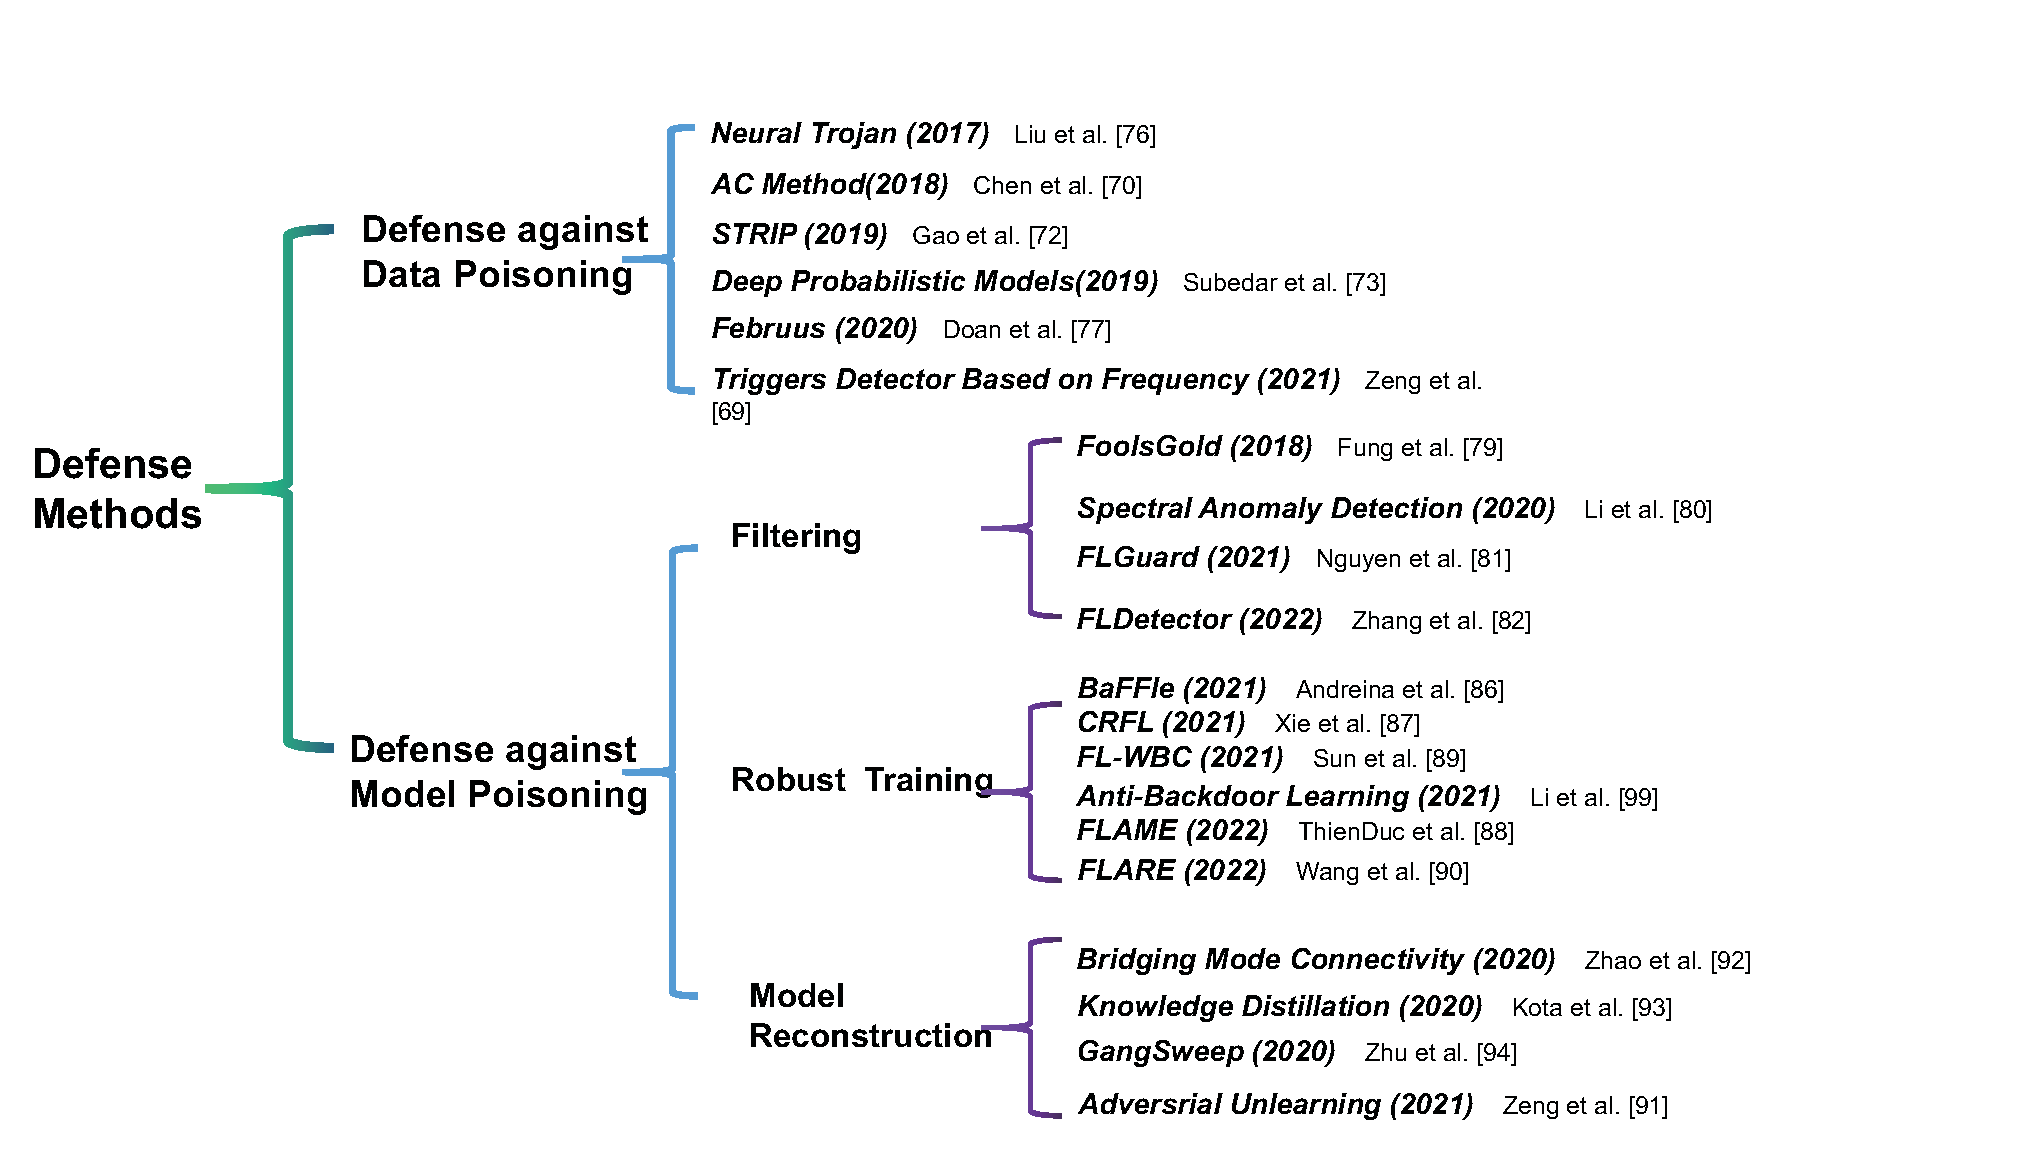
\includegraphics[width=1.0\linewidth,height=3.5in]{output/fig8.eps}
     \caption{This graph is a summary of some of the defensive solutions mentioned in this article, we have summarized and categorized some
     of them in this graph, and sorted them in chronological order.}
     \label{fig8}
\end{figure*}

To mitigate the problem of backdoor attacks in
federated learning, various defensive techniques have been
proposed. As shown in Fig.~\ref{fig8}, given that we previously
categorized backdoor attacks as data poisoning attacks
and model poisoning attacks, we will now discuss defensive
strategies for each of these attack types.  

\subsection{Defense against Data Poisoning}  
The simplest approach is to filter out poisoned data
samples, which aims to remove the poisoned samples from
the training datasets. After the filtering process, only
benign samples or purified poisoned samples are used
during the training process, thus eliminating the creation
of backdoors from the source.  

Tran et al.~\cite{tran2018spectral} are the first to investigate methods
for filtering out malicious samples from the training sets.
They demonstrate that poisoned samples tend to leave
detectable traces within the covariance range of the feature
representation. Exploiting this insight, it is possible to
filter out poisoned samples from the training sets. Chen et
al.~\cite{chen2018detecting} propose a two-stage filtering approach. As shown
in Fig.~\ref{fig9}, in the first stage, activation values of samples
in each class are clustered into two groups. And in the
second stage, it is determined which clusters correspond
to poisoned samples. This method is the first methodology
for detecting poisonous data maliciously inserted into the
training set to generate backdoors that does not require
verified and trusted data. It has been released as a part
of the IBM Adversarial Robustness ToolBox. Similarly,
Zeng et al.~\cite{zeng2021rethinking} reveal that poisoned samples of existing
attacks have some high-frequency artifacts even if their
trigger patterns are invisible in the input space. Based on
this observation, they design a simple yet effective filtering
method based on those artifacts. Based on data-driven defense methods, in addition
to filtering out samples, it is also possible to consider
directly preprocessing the samples, specifically by erasing
any backdoors within them to prevent them from being
embedded in the model. Liu et al.~\cite{liu2017neural} propose a 
pretrained autoencoder as a preprocessor to prevent malicious
samples from embedding backdoors by preprocessing the
input samples without affecting data classification accuracy.  

Doan et al.~\cite{doan2020februus} propose a two-stage image processing
method called Februus, in which, in the first stage, Februus
uses GradCAM to identify influential regions, which are
then removed and replaced with neutral color frames.
Subsequently, as shown in Fig.~\ref{fig10}, Februus uses a GAN-based
repair method to reconstruct the masked regions
to mitigate their adverse effects (such as benign accuracy
reduction). Li et al.~\cite{li2021backdoor} discuss the properties of existing
poisoning-based static trigger mode attacks. They 
demonstrate that the attack performance may sharply decrease
if the appearance or location of the trigger is slightly
changed. Based on this observation, they recommend using
spatial transformations (such as contraction, flipping) for
defense. Compared to previous methods, this method is
more efficient because it requires almost no additional
computational cost.  

\subsection{Defense Against Model Poisoning}  
(1)Filtering: Similar to defense methods against
poisoned data, defense methods against poisoned models also
begin with model filtering. Fung et al. propose FoolsGold~\cite{fung2018mitigating}
, which checks for and eliminates suspicious updates
during local updates. FoolsGold is based on the fact that
when a global model is trained by a group of attackers,
they will submit updates with the same backdoor objectives
throughout the training process, resulting in similar behaviors.  

\begin{figure}[h]
    \centering
    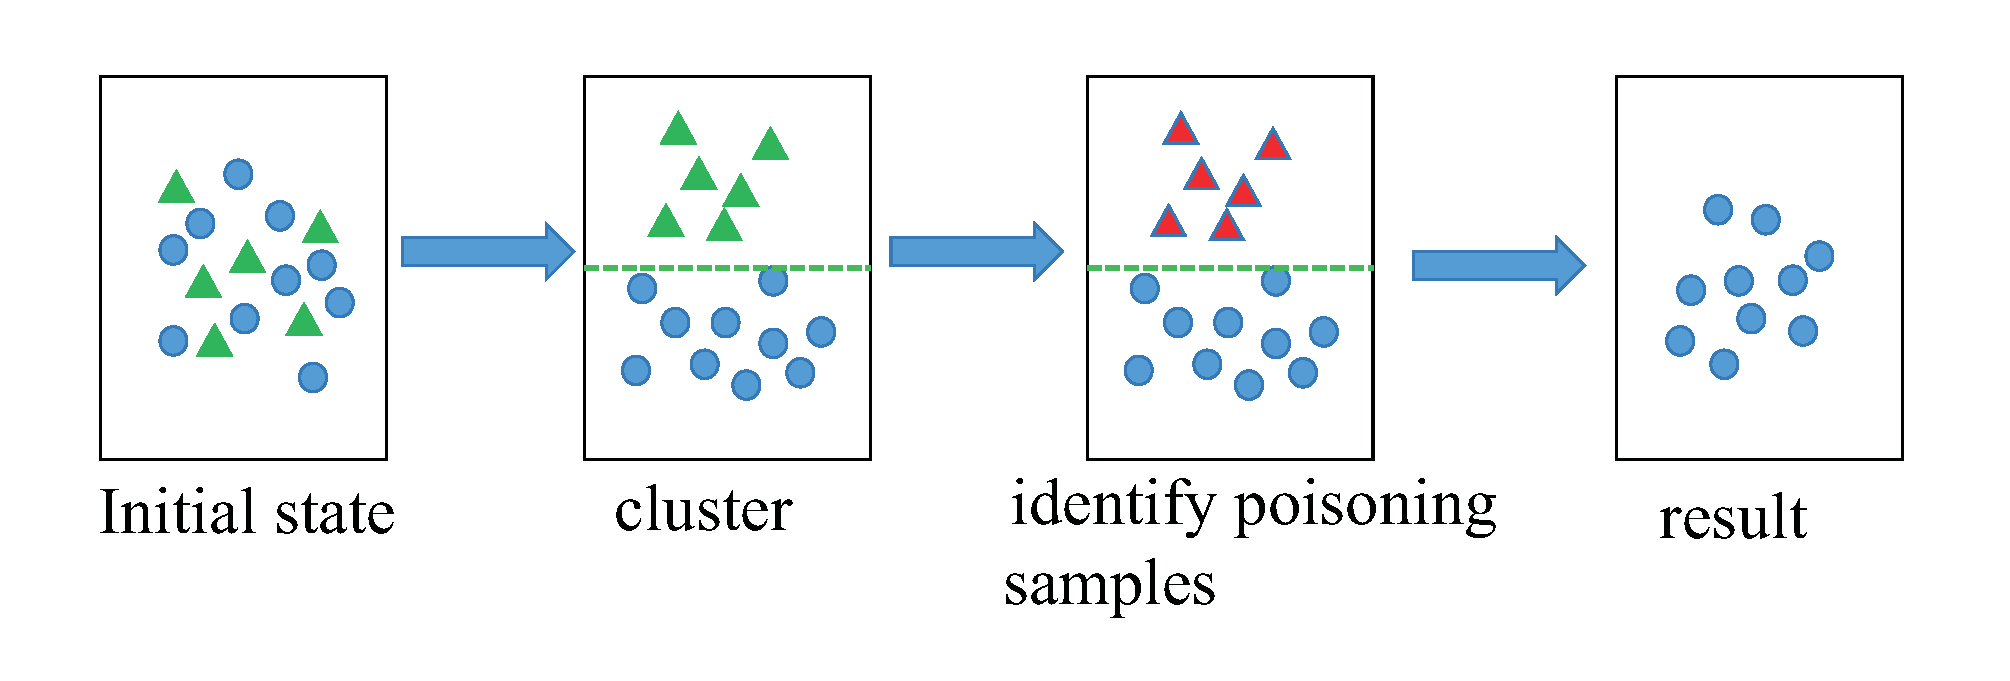
\includegraphics[width=1.0\linewidth,height=1.0in]{output/fig9.eps}
     \caption{In the first stage, activation values of samples in each class are
     clustered into two groups. And in the second stage, it is determined
     which clusters correspond to poisoned samples.}
     \label{fig9}
\end{figure}

However, this similarity does not occur among honest
participants because each user’s training datasets are
unique and not shared with others. Therefore,
malicious attackers can be separated from benign attackers
through gradient updates. After detecting such anomalies,
FoolGold maintains the learning rate of benign users
(submitting only unique gradient updates) and reduces
the learning rate of malicious users (repeatedly uploading
similar gradient updates) to mitigate backdoor attacks.
However, experimental results show that FoolsGold cannot
defend against adaptive attacks.  

\begin{figure}[h]
    \centering
    \includegraphics[width=1.0\linewidth,height=2.0in]{output/fig10.eps}
     \caption{Februus uses a GAN-based repair method to reconstruct
     the masked regions to mitigate their adverse effects (such as benign
     accuracy reduction).}
     \label{fig10}
\end{figure}

Li et al.~\cite{li2020learning} propose a spectral anomaly detection
framework for a central aggregator that detects and
erases malicious updates through strong detection model
detection. The key idea of spectral anomaly detection
is that there is a significant difference between the
embedding of benign updates and backdoor updates in
a low-dimensional latent space. One practical method
for approximating low-dimensional embedding is to build
a model using an encoder-decoder structure, where the
encoder takes in the raw update and returns a low
dimensional embedding, and the decoder is fed the embedding and outputs the generation error.
After training the encoder-decoder model on benign updates, it can
be used to identify backdoor updates, generating errors
much higher than benign errors; malicious updates will
be excluded from the aggregation process. However, this
defense method cannot handle multi-trigger backdoor
attacks, i.e., injecting various backdoors simultaneously.  

Nguyen et al. propose FlGuard~\cite{nguyen2021flguard}, a two-layer defense
method that checks for locally updated updates with
clear backdoor effects and eliminates residual backdoors
through pruning, smoothing, and noise addition. Unlike
FoolsGold~\cite{fung2018mitigating}, it also applies to multi-trigger backdoor
attacks while maintaining high prediction accuracy for
benign primary tasks. Additionally, FLDetector~\cite{zhang2022fldetector}
proposes a method to detect malicious clients by checking
the consistency of model updates. Essentially, the server
predicts the clien's model update based on past updates
in each iteration. If the model update received by the
client differs significantly from the predicted update over
multiple iterations, the client is marked as malicious.
Overall, the focus of these methods is mainly divided
into two types: the first is to remove toxic updates
from malicious clients before model aggregation, and the
second is to reduce the impact of malicious clients on the
aggregated model, such as reducing the learning rate of
suspicious clients.  

(2)Robust Training: After filtering techniques, another
class of techniques aims to directly mitigate backdoor
attacks during model training through robust joint training.
Differential privacy algorithms have been shown to be
effective against backdoors~\cite{naseri2020toward}, but they may compromise
model performance under data imbalance commonly found
in federated learning~\cite{bagdasaryan2019differential}. DP-FedAvg~\cite{mcmahan2017learning} (Central-DP)
is a differential private aggregation strategy that
eliminates outliers by clipping the norm of model updates
and adding Gaussian noise, but the required amount of
noise significantly reduces task accuracy. Sun et al.~\cite{prakash2020mitigating} 
proposed weak DP, which adds sufficient Gaussian noise to
defeat backdoors while maintaining task accuracy, but it is
ineffective against constraint-based backdoor attacks~\cite{li2023federated} .
Additionally, DP-based defenses can potentially impact
the benign performance of the global model, as the
clipping factor also changes the weights of benign model
updates.  

In addition to DP-based defenses, Andreina et al.~\cite{andreina2021baffle}
propose Feedback-based Federated Learning (BaFFle)
to eliminate backdoors. The key idea of BaFFle is to
leverage participants to verify the global model. BaFFle
includes a super-digit verification process for each round
of federated learning. Specifically, each selected
participant checks the current global model by computing a
verification function on their secret data and reports to
the central server whether the model is backdoored or
not. The central server then decides whether to accept or
reject the current global model based on feedback from all
users. The verification function compares the error rate of
a specific class of the current global model with the error
rate of previously accepted global models. If the error
rate is significantly different, the central server rejects the
current global model as it may be backdoored and issues
an alert. Unlike anomaly detection, BaFFle is compliant
with secure aggregation.  

\begin{figure}[h]
    \centering
    \includegraphics[width=1.0\linewidth,height=2.5in]{output/fig11.eps}
     \caption{Overview of certifiably robust federated learning (CRFL).
     CRFL controls the model smoothness through pruning and smooth-
     ing of model parameters and generates sample robustness certifica-
     tion against amplitude-limited backdoor attacks. Smoothness and
     perturbation methods are also used as additional components to
     constrain the L2 norm of individual updates to enhance defense
     performance.}
     \label{fig11}
\end{figure}

Considering that all of the above defense works lack
robustness certification, Xie et al.~\cite{xie2021crfl} propose the first
general defense framework CRFL for training certifiably
robust FL models against backdoor attacks. As shown
in Fig.~\ref{fig11}, CRFL controls the model smoothness through
pruning and smoothing of model parameters and generates
sample robustness certification against amplitude-limited
backdoor attacks. Smoothness and perturbation methods
are also used as additional components to constrain
the L2 norm of individual updates to enhance defense performance~\cite{nguyen2022flame}.
In addition, the FL-WBC~\cite{sun2021fl} method aims to identify
the fragile parameter space in FL and perturb it during
client training. FL-WBC also provides robustness
guarantees against backdoor attacks and convergence guarantees
for FedAvg. These developments demonstrate promising
steps toward improving FL's robustness against backdoor
attacks. In FLARE~\cite{wang2022flare}, a trust evaluation method is
proposed that calculates a trust score for each model
update based on the difference between all model updates
and their penultimate layer representation values. FLARE
assumes that most clients are trustworthy and assigns
low scores to updates that are far from benign update
clusters. The model updates are then aggregated with their
trust scores as weights and the global model is updated
accordingly. In~\cite{li2021anti}, the concept of anti-backdoor learning is
introduced, which involves training a clean model given
infected data, dividing the overall learning task into a
dual task of learning the clean part of the data and
the backdoor part. The article leverages two inherent
weaknesses of backdoor attacks: models learn backdoor
data faster than clean data, and the stronger the attack,
the faster the model converges on the backdoor data.
Additionally, backdoor tasks are mutually associated with
specific classes. Based on these two weaknesses, a generic
learning scheme is proposed to automatically prevent
backdoor attacks during training. A two-stage gradient
ascent mechanism is introduced to isolate and separate
backdoor samples from the target class during the early
training stage and break the association between backdoor
samples and the target class during the later training
stage.  


(3)Model Reconstruction: The model reconstruction-based
approach aims to eliminate hidden backdoors in infected
models by directly modifying suspicious models.
Therefore, even if triggers are included in the attack
samples, the reconstructed model will still correctly predict
them because the hidden backdoors have been removed. As mentioned earlier, the forgetting mechanism of
federated backdoor attacks means that as training and
model aggregation progress, the backdoor will be forgotten
in successive iterations. As a defense, this forgetting
mechanism can also be utilized to create many defensive
methods. Zeng et al.~\cite{zeng2021adversarial} define multiple training as a min-max
problem and used implicit hyper-gradients to explain the
interdependence between internal and external optimization.
In~\cite{zhao2020bridging}, Zhao et al. show that hidden backdoors
infecting DNNs can be repaired using pattern connectivity
techniques with a certain number of benign samples. Li et al.~\cite{yoshida2020disabling} perturb backdoor-related neurons based
on the distillation process, reconstructed (infected) DNNs
using knowledge distillation techniques, and
thus removed hidden backdoors. Huang et al. ~\cite{huang2023distilling} propose a
distillation technique that utilizes Cognitive Distills to
extract Cognitive patterns. This is because the patterns of
backdoor examples are generally small and sparse, making
it possible to detect poisoned examples.  

In addition to directly eliminating hidden backdoors,
defense based on trigger synthesis first synthesizes
backdoor triggers, and then in the second phase, eliminates
hidden backdoors by suppressing the influence of triggers.
These defenses have some similarities in the second phase
with reconstruction-based defenses. For example, pruning
and retraining are commonly used techniques to remove
hidden backdoors in both defenses. However, compared to
reconstruction-based defenses, the trigger-based defenses'
trigger information makes the removal process more effective and efficient.  

A GAN-based method is proposed in~\cite{zhu2020gangsweep} to synthesize
trigger distributions. In~\cite{guo2020towards}, they show that the detection
process used in~\cite{wang2019neural} to determine synthesized triggers has
several failure modes and proposed a new defense method
based on this observation. Additionally, Cheng et al. ~\cite{xu2020defending}
reveal that the $\infty$ norm of activation values can be used to
distinguish backdoor-related neurons based on synthesized
triggers. Therefore, they propose performing an $\infty$-based
neuron pruning to remove neurons with high activation
values in response to triggers. Similarly, Aiken et al.~\cite{aiken2021neural} 
also propose removing hidden backdoors by pruning DNNs
based on synthesized triggers from another perspective. 

In general, we do not consider filtering techniques to be
a viable solution for mitigating backdoor attacks. Because
filtering technologies are generally designed for specific
types of attacks, they can be easily spoofed by attackers.
Instead, we believe that the focus of research on backdoor
defense should be on model reconstruction and robust
training.